\chapter{Interactive Segmentation for Textureless Objects}
\label{chapter:Textureless Segmentation}


\section{System Pipeline}
%\subsection{Static Segmentation - Preprocessing}

\begin{figure}[h!]
\centering
  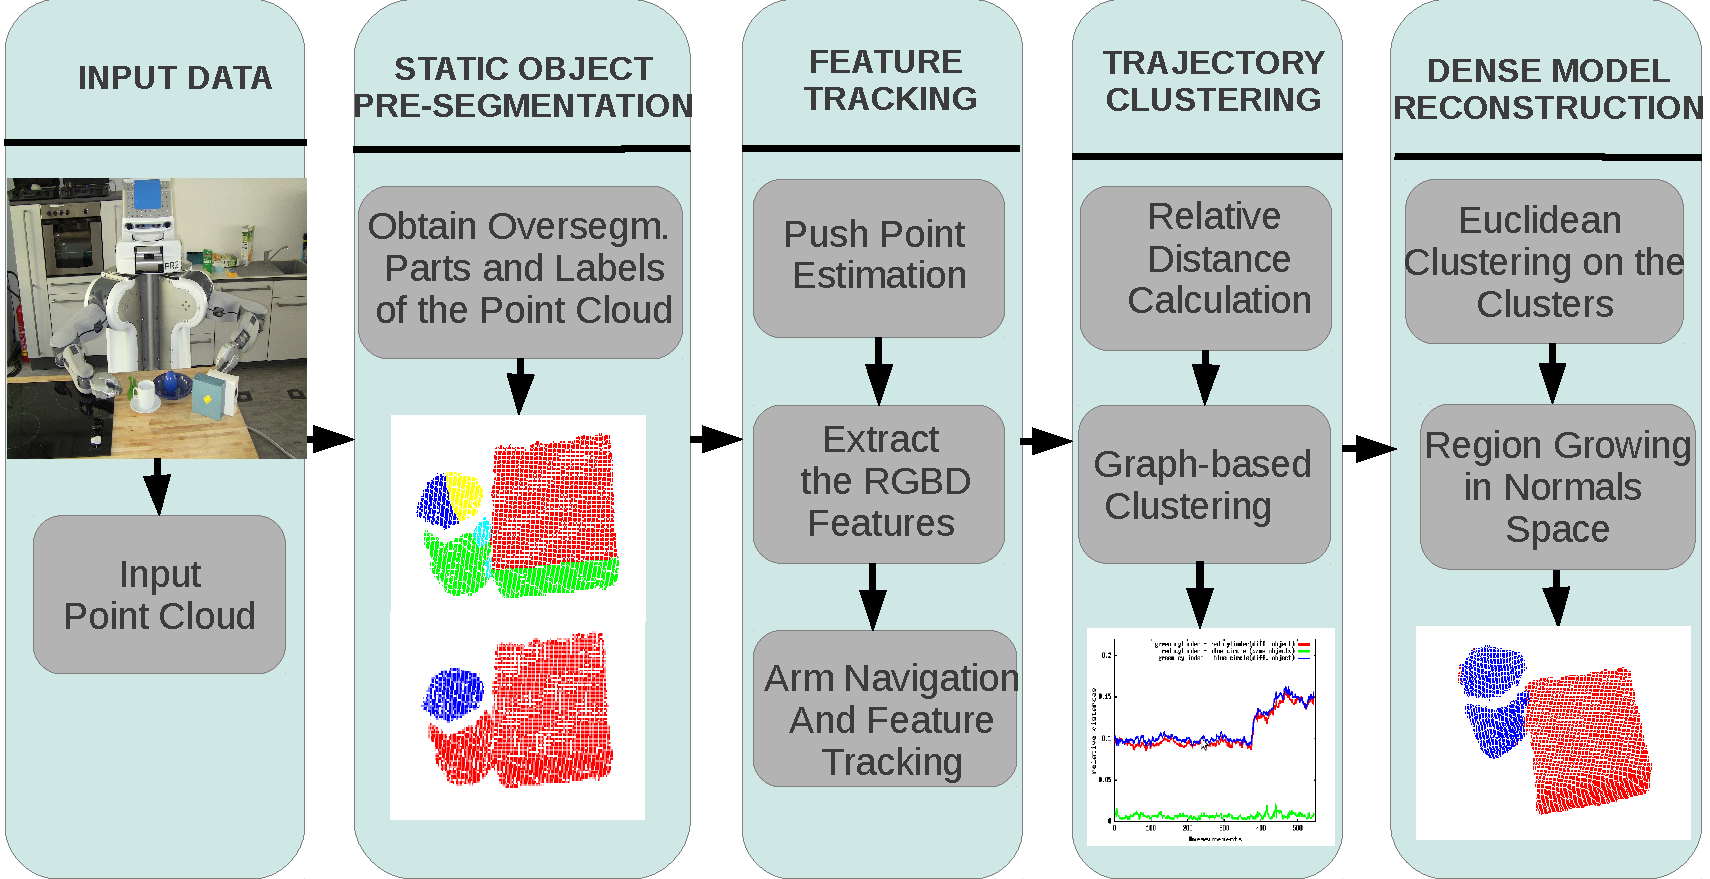
\includegraphics[width=\columnwidth]{figures/segmentation_pipeline.pdf}
  \caption{System pipeline.}
  \label{fig:pipeline}
\end{figure}


\begin{figure*}[ht!]  %\renewcommand*{\thesubfigure}{}
  \begin{centering} 
    \begin{tabular}{p{0.166\textwidth}p{0.166\textwidth}p{0.166\textwidth}p{0.166\textwidth}p{0.166\textwidth}p{0.166\textwidth}}
    \includegraphics[height=1.65cm]{figures/scene1/image_before.jpg}
&    \includegraphics[height=1.65cm]{figures/scene1/pcl_before.png}
&    \includegraphics[height=1.65cm]{figures/scene1/segments.png}
&    \includegraphics[height=1.65cm]{figures/scene1/labels.png}
&    \includegraphics[height=1.65cm]{figures/scene1/pcl_after.png}    
&    \includegraphics[height=1.65cm]{figures/scene1/distances.png}\\

    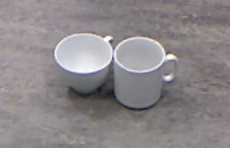
\includegraphics[height=1.65cm]{figures/scene2/image_before1.jpg}
&    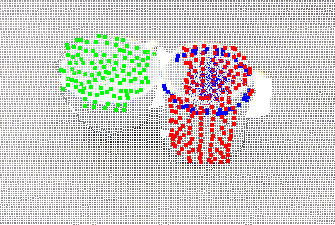
\includegraphics[height=1.65cm]{figures/scene2/pcl_before1.png}
&    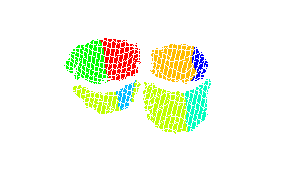
\includegraphics[height=1.65cm]{figures/scene2/segments1.png}    
&    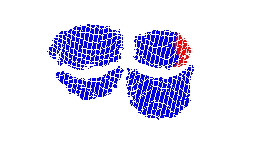
\includegraphics[height=1.65cm]{figures/scene2/labels1.png}
&    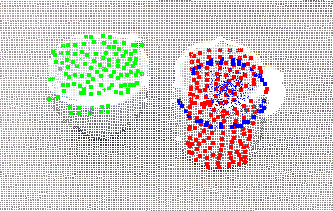
\includegraphics[height=1.65cm]{figures/scene2/pcl_after1.png}  
&    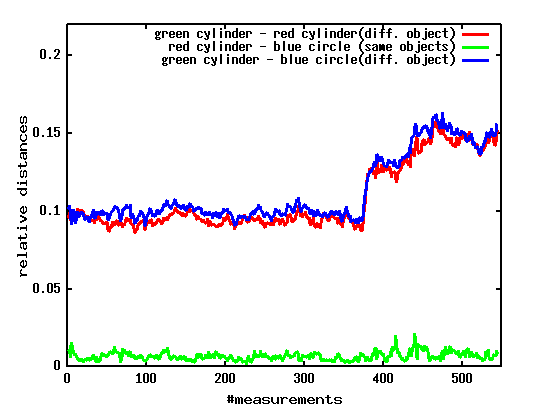
\includegraphics[height=1.65cm]{figures/scene2/distances.png}

%     \includegraphics[height=1.65cm]{scene3/image_before.jpg}
% &    \includegraphics[height=1.65cm]{scene3/pcl_before.png}
% &    \includegraphics[height=1.65cm]{scene3/segments.png}
% &    \includegraphics[height=1.65cm]{scene3/labels.png}
% &    \includegraphics[height=1.65cm]{scene3/pcl_after.png}    
% &    \includegraphics[height=1.65cm]{scene3/distances.png}
  \end{tabular}
		\vspace{-2ex}
    \caption{Two test scenes in the top and bottom row respectively. First column:
      original scenes; second column: extracted RGBD features before the
      interaction; third column: parts $P$ from the static segmentation;
      fourth column: object hypotheses $O$ from the static segmentation; fifth column:
      tracked RGBD features after interaction; sixth column: relative
      distances between the tracked features. Plots with the ramp denote distances between features on different objects 
      and plots with the constant values denote distance between features on the same object.}
    \label{fig:scenes}
  \end{centering}
\end{figure*}


 The approach taken to segment textureless objects   
 consists of five main steps as depicted in Fig. \ref{fig:pipeline}
  and demonstrated in a video\footnote{\url{http://youtu.be/Bu4LayrGC1s}}.
 In the first step we obtain an RGBD point cloud from the Kinect sensor. In the second step we perform static object
 pre-segmentation which results in a set of categorized object hypotheses $O$,
 with the category being either flat or round, and a list of object parts $P_{o}$ that every object 
 $o \in O$ consists of. Having obtained the object hypotheses $O$ we infer which hypothesis
 is segmented  correctly. For
 that we count the  number of parts that the respective object hypotheses $O$ 
 consists of and then sample from the Poisson distribution according to the Eq. \ref{eq:poisson}.
 After obtaining the probability of the scene being segmented correctly we 
decide if the interactive segmentation algorithm should be used or not. It is worth mentioning that the system is able to perform with a different static segmentation algorithm that could be used as an indicator if we need to use the interactive segmentation algorithm.



 The information obtained from the categorization algorithm is also used in the next step - based on the object category we decide what kind of RGBD feature needs to be extracted and tracked afterwards. Having obtained one of the categories being flat or round, we extract different RGBD features: lines and corners for the flat objects or cylinders and circles for the round ones. As the next step we look for the best point to push the objects by looking at concave and convex corners in a top-down image of the scene and we execute the arm motion movement at the previously found corner. We move the arm in $1cm$ intervals until we reached a maximum of $5$ 
  pushes. All of the features are being tracked during the interaction 
 and the trajectories of feature centroids  are being  saved as 6 degrees of freedom transformations. 
 
  
%In sixth  row of  \figref{scenes} the
% relative distances between centroids over the time are depicted. 
In the fourth step we apply a graph-based algorithm for trajectory clustering that operates on the saved centroids mentioned above. At the end of this step we obtain a set of grouped features where each group of features is considered to belong to the same object. In this way features that have moved in the same manner are clustered as one feature. 

 In the fifth and the last step the dense model is reconstructed using the region growing algorithm 
where the centroids of tracked and clustered RGBD features are
used as seed points. As an output we obtain a dense representation of the objects in the scene that may be further used for grasping or object recognition algorithms.

\section{Pre-processing Steps}


\subsection{Static Pre-segmentation of Objects}
\label{sec:static-seg}

% As a first step we want to to segment our static scene in flat and round objects.
In order to achieve a pre-segmentation we make use of the classification method presented 
in~\cite{marton12SC} based on part-graph-based hashing.
The basic idea is that segmenting objects accurately 
in a cluttered scene does not always yield the expected result, as seen in %\figref{scenes} 
column 4, and can lead to classification failures, 
but over-segmenting is easily realizable~\cite{soupofsegments,Lai_Fox_2010,mozos11furniture}. 
We use the classification approach described in~\cite{marton12SC} 
for categorizing over-segmented object parts in cluttered scenes
by considering combinations of these parts to compute features
and classify these efficiently with the aid of hashing.
The result is a set of labeled parts with geometric categories
that can be grouped in order to obtain object hypotheses.
Based on statistics computed from the training data on single objects, 
we can estimate how likely it is that an object hypothesis is
correct.

%\textbf{Why using a categorization algorithm for pre-segmentation?}
%In \figref{segmentation_comparison} we have alluded to the fact that it
%is close to impossible to recover the failure cases since the graph-based
%segmentation algorithm as well as the region growing one work on the level
%of pixels and points in the point cloud. Part-graph-based hashing algorithm on
%the other hand is a learning-based algorithm that bears the semantic of the 
%object categories with it. In this particular case we are thus able to collect
%the statistics about the probable number of parts one object is composed of in 
%the training stage and then deduce whether the categorization of a given scene is 
%likely correct or not.

In the rest of the section we summarize the part-graph-based 
hashing algorithm briefly and show how we use it to guide
%turn it into a ``rich'' pre-segmentation algorithm that guides
the interactive segmentation.

\subsubsection{Decomposition into Part Graphs}
\label{sec:part-graphs}
In order to find the parts ($p_{1}, \dots, p_{n} \in P_{o}$) 
in the point clouds we use the clustering criteria presented in~\cite{mozos11furniture},
such that patches with a small curvature are considered, as shown in
%\figref{scenes} 
REF
column 3.  For each part we subsequently compute GRSD- (Global Radius-based 
Surface Descriptor~\cite{irosws11vosch}) feature and store it for later use. We then 
extract the part neighborhoods by checking if the physical distance between two 
parts falls below a threshold of $2cm$ (considering Kinect noise level~\cite{kinect_accuracy}), and build a connectivity matrix. 
Starting at each vertex of the connectivity matrix, we create all the possible groupings up to a certain size 
(eight parts in the case of single objects and four in the case of cluttered scenes) 
in order to obtain the ``soup of segments'', and create the groups' hash codes
using isomorphic graph metrics. The hash codes are then used to further split the feature 
space ending up with a separate classifier (nearest neighbors in our case) for each hash code. 
During the classification phase we obtain confidence votes only from those classifiers,
which were created for the hash codes that are found in our scene. Based on these votes
a decision is made upon the class of the segments. For a detailed description of this approach 
please refer to~\cite{marton12SC}.

% For the hash codes, apart from the number of vertices/parts, we chose to concatenate the 
% sorted list of vertex degrees as well to form a second level of keys. As an alternative 
% for this second level of keys we experimented with using the eigen values of the graph's 
% Laplacian matrix, but found that the results upon evaluation were the same. 
% For this reason, in the upcoming testings and evaluations we used the sorted list of vertex 
% degrees, as they are simpler to compute. This degree order is unique for isomorph graphs, 
% however different graphs can have the same degree order.

% We use a region-growing approach, that starts at a random point
% and grows the segment until the deviation from the seed normal does not exceed 45 degrees.
% This way, selecting different seed points result in multiple segmentations of the point cloud into parts.
% This process is not completely reproducible, therefore authors in \cite{marton12SC} rely on the
% large amount of training data to cover all possible cases. 
% Since we are dealing with tabletop scenes, the supporting plane 
% can be removed prior to processing, and only points above it 
% considered as in \cite{marton11ijrr}. 

% Note that since the graph vertices can be sorted, it is possible to efficiently 
% enumerate all sub-graphs containing a given vertex without repeating already generated ones.

\subsubsection{Object Part Categorization}
\label{sec:part-feature}
The classifier was trained on a subset of the dataset from~\cite{lai11db} 
as presented in~\cite{marton12SC}.
The choice of the feature determined for each part, namely the GRSD- is motivated 
by the fact that we are dealing with novel objects not seen before 
by the classifier, so in order to successfully categorize them we need to use geometric features.
% As described in \cite{irosws11vosch}, we adapted the GRSD feature to be additive, 
% by simplifying it to simple histogram of neighborhoods of surfaces of different type,
% neglecting the ray-tracing step. We evaluated the GRSD- feature on the same dataset 
% and in the same manner as described in~\cite{marton12SC}.
Additionally, the low dimensionality and additive property\footnote{If the feature is additive,
the descriptor that would be computed for the object is the same as the sum of the features of its segments.} make GRSD- a suitable choice for such task.

Objects ($o_{1}, \dots, o_{n} \in O$) are categorized in six geometrical categories: sphere, box, rectangular/flat, cylinder, disk/plate and other.
Doing this we get a better a discrimination between different objects. After having the results for the 
six geometrical classes, we merge them together into different \emph{object types} considering everything spherical and cylindrical being
\emph{round}, and disks/plates, flats and boxes as \emph{flat} objects.
With the category \emph{other} we thus get three object types, whereas most
household objects fall into the first two~\cite{marton11ijrr}.

In this paper we omit the category \emph{other} and use the other two in order
to determine if the interactive segmentation is needed, and if yes, which RGBD features 
to extract and track in the respective part of the point cloud in the given scene.

\subsubsection{Verification of Correctness of Segmentation}
\label{sec:probabilities}	
Since the geometric categorization of parts does not give the correct grouping of these parts to form objects,
simply grouping the parts of the same category together does not always separate the objects, especially if classification errors occur too.
A method of voting for object centroids followed by a model fitting step was described in~\cite{mozos11furniture},
but we assume having no CAD models for test objects in this paper. We would also have to consider 6DOF poses, complicating the approach considerably.

Whereas the segmentation of objects is not uniquely defined, there are still regularities in the number of parts they are broken up into.
As shown in REF%\figref{poisson}
, the distribution of the number of different object parts, generated in the training stage of the part-graph-based hashing algorithm, can be modeled as a Poisson distribution,
with an average error of 1.7\% (and at most roughly 9\%).


The Poisson distribution described by REF%\equref{poisson} 
describes the probability of different number of events occurring
in a given interval, which we interpret here as the number of part boundaries encountered over the surface of the scanned object.
The parameter $\lambda$ is the mean of number of parts, which in our case is 0.876 for flat, 2.166 for round, and 3.317 for other object types.
\begin{equation}
\label{eq:poisson}
P(k~parts~forming~a~single~object) = \lambda^k \exp{-\lambda} / k!
\end{equation}

This simple model is used to judge if a group of parts of the same geometric category forms a single object or if the robot
should try to interact with it. We cut the probabilities at $0.3$ for flat and $0.15$ for round objects.

\textbf{Example:} To demonstrate this, from the right part of %\figref{poisson} 
we can deduce that the 
flat object is most likely to consist of 1 or 2 parts. The test scene with 
2 boxes REF %(\figref{scenes}) 
was categorized as one object (column 4), but in column
3 we notice that there are 6 parts in the scene. The probability for 1 object consisting of 6 parts is below the $0.3$ value
according to the Poisson distribution and clearly indicates an over-segmentation 
error and the need for the robot to segment this region interactively.

\begin{figure}[h!]
\centering
  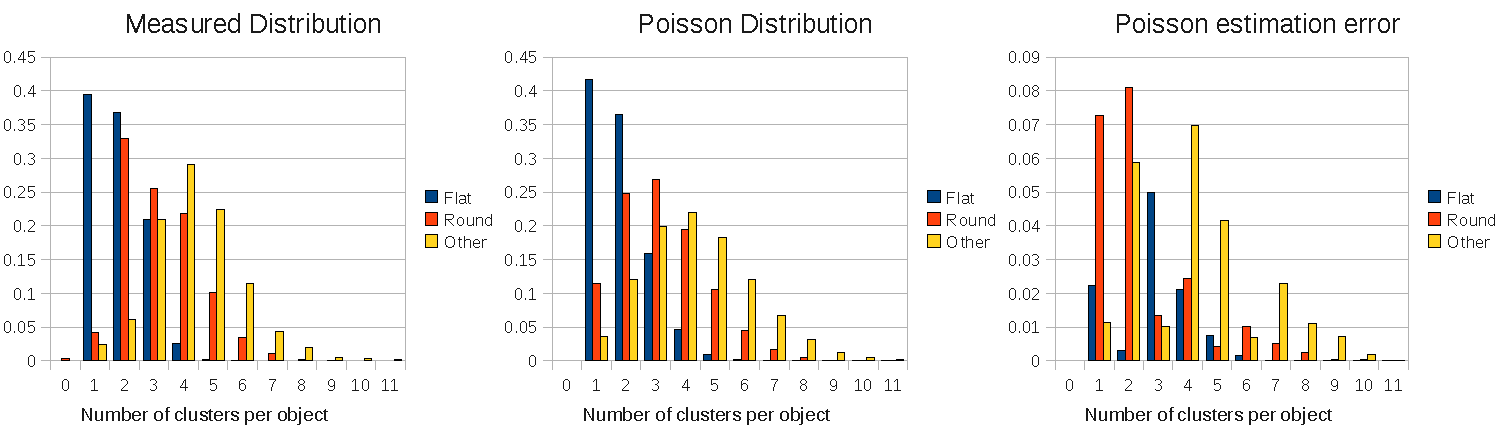
\includegraphics[width=0.98\columnwidth, trim=0ex 0ex 53ex 0ex, clip]{figures/dataset_stats.pdf}
	\vspace{-2ex}
  \caption{Distribution of number of parts (see REF column 3) per object and their approximation with a Poisson distribution.}
  \label{fig:poisson}
\end{figure}

\subsection{Push Point Estimation}
\label{sec:push-point}
Once the over or under segmented region of interest has been identified 
according to the above generated distribution, the  appropriate contact
points  between the objects in   the   scene  and   the   robot's   end   
effector  must   be determined. Furthermore, the  direction   the robot's  end
effector should move must be chosen.

The contact points where the objects are pushed should
be such that the push results in different objects moving
differently resulting in different optical flows.
In  this thesis we apply our previously developed approach based on 
the local concavities~\cite{bersch12interactive}. The outcome
of a push depends largely on the arrangement of objects but
intuition suggests that pushing at corners of objects should
result in not only translation but also rotation of the object
directly being pushed. On the other hand, pushing at the
sides of an object may result only in translation and any
neighboring objects may also move together with it as a
rigid body. Object corners are, therefore, good candidates for
contact points for pushes irrespective of the object configura-
tion. Also, since most
commonly  encountered  household   items  have  convex  outlines  when
observed  from  above,  our  system  uses  local
concavities in the  2D contour of an object group  as an indicator for
boundaries between the objects.
We use this heuristic to select our push points and later
validate the accuracy of this heuristic through simulations in
the next section.

\begin{figure}[tb!]
   \begin{center}
     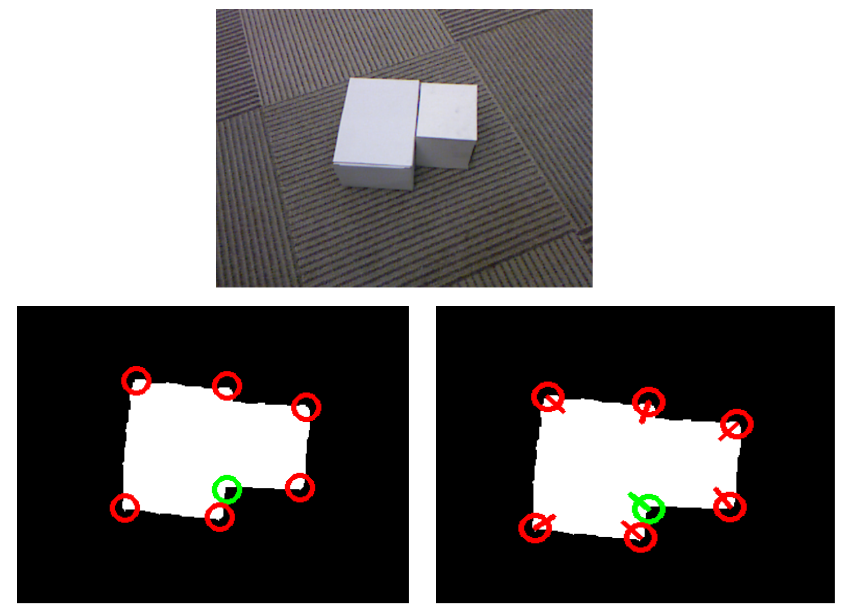
\includegraphics[width=.9\columnwidth]{figures/corners.png}
		\vspace{-2ex}
   \caption{Corners and their directions after morphological operations. 1st row - image of the scene. 2nd row, 1st column - Corners detected from the top-view image. 2nd row, 2nd column - Directions detected from the top-down image. }
   \label{fig:corners}
 \end{center}
 \end{figure}

In order to detect concave and convex corners we developed the following algorithm. Firstly we artificially translate and rotate the camera image such that it looks as taken directly from above the scene. From this point an image and a point cloud are taken to determine potential push points for the robot. Having the point cloud information we use Plane Segmentation algorithm from the Point Cloud Library(pointclouds.org) to segment the biggest plane in the scene - a table. We refine the images by using simple morphological operations - opening and closing. After these steps we obtain black and white images where everything but objects is black, an example is depicted in Fig. \ref{fig:corners}. 

Taking this image as an output we use Shi-Tomasi corner detector to determine corner positions and their orientation. As the implementation details of the corner-based pushing go beyond the scope of this thesis, we refer the reader to~\cite{bersch12interactive} for details.

\subsubsection{Push Point Heuristic Validation}
We carried  out several simulations  in physics-based simulator Gazebo\footnote{\url{http://gazebosim.org/}} to validate  our corner
pushing heuristic. To verify that  pushing at corners is  indeed more
effective, we  spawned different  scenes in Gazebo  with two  or three
closely  placed objects. Objects were flat and round, in different orientations 
and arranged such that they were in solid contact or in single point contact.
We  then simulated  pushing at  these objects
with a PR2 gripper at many different contact points along the bounding
box of the  objects and in many different  directions. More precisely,
we chose points along the bounding box spaced $2cm$ apart and for every
such  point,  the  gripper simulated  a  sequence  of  2 pushes  in  7
different directions {15\textdegree}  apart (See Fig.~\ref{fig:simulations}). The starting gripper pose
and the object  poses before and after every  push were recorded. Then
Shi-Tomasi features with known but randomly determined  locations were spawned artificially on
the objects. Based on the  recorded object poses, the locations of all
the  features were  computed  after  every push.  This  enabled us  to
compute the simulated optical flows. The feature trajectories  so obtained were
then clustered using our previously developed segmentation for textured objects algorithm.
We used this algorithm because of the character of the features - there are many different forms of textureless features and it is difficult to come up with a general solution whereas Shi and Tomasi features are a good representatives for many textured tracking algorithms.  The contact points for the
pushes  which resulted in  a successful  segmentation of  objects were
then  observed  and  the  number  of  successful  corner  pushes  were
counted. A push  was classified as a corner push  if the contact point
is less than $1cm$ away from an object corner.

\begin{figure}[h!]
  \begin{center}
    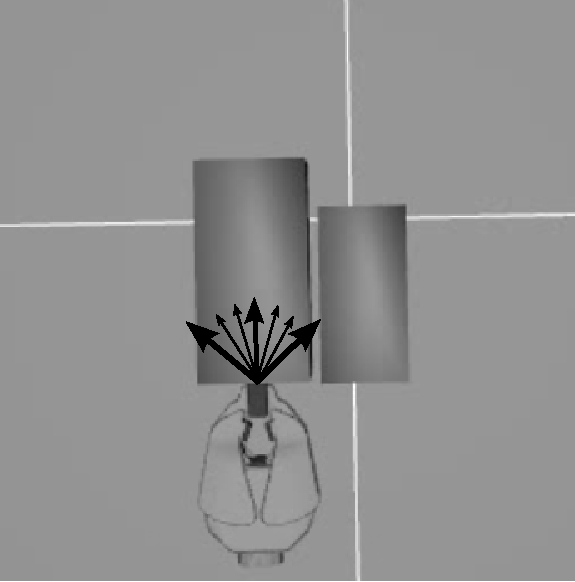
\includegraphics[width=0.2\textwidth]{figures/push_directions.pdf}  
    \includegraphics[width=0.2\textwidth]{figures/rviz_empty9_crop.pdf} 
    \caption{Screenshots from  the Gazebo  simulation of a  two object
      scene (left)   and  the   corresponding  visualization   of  the
      segmentation result. The black arrows in the left image show the
      7 push  directions for a single  contact point. The  dots on the
      objects in  the right image represent features  and their colors
      represent  the cluster they  were assigned  to for  a particular
      successful push sequence. The red arrows represent the starting gripper positions
      and  directions  of  all  the  successful push  sequences  in  a
      simulation run. }
         \label{fig:simulations}
  \end{center}
\end{figure}

We carried out 5 runs\footnote{Please mind that since Gazebo uses an ODE engine 
which is based on linear complementarity problem constraint formulation and since the
simulation is defendant on the CPU load, the runs are not fully deterministic.} 
on every of 24 different  scenes (11 scenes  with 2
objects, 13  scenes with  3 objects), which resulted in an average  of 381.5
push sequences for a scene out of which an average of 14.9 pushes were
successful in segmenting  all the objects in the  scene correctly. Out
of these, 7.25  pushes were corner pushes. There were an average  of 10
object corners in each scene. From this it follows that there were on average
70 corner pushes and 311.5 other pushes. This gives the segmentation success of $10\%$
for the corner pushes and $2.4\%$ for the non-corner ones. The reason for the low
overall segmentation result compared to the real scenes above is on the one hand in that the scenes in the simulation
included the single contact points between the objects and on the other hand in 
that various non-favorable orientations per contact point were computed and executed.
We observed  that corner pushing was successful  in all  the scenes while  side pushing  was successful
only  when  the  objects were in single point contact. 
When the  objects were next to each other  and similar in size,
pushing  at the sides  resulted in  the objects  moving together  as a
single rigid body, thus making the algorithm fail. In such cases, only
corner  pushes succeeded.  These simulations  thus prove the benefits of
corner pushing irrespective of object arrangement.



\section{Textureless Object Segmentation}
\label{sec:textureless}

The main challenge in dealing with textureless objects is finding good and stable features. In our approach we decided to take use of the information we have from the previous steps namely the category of the object. Since there is no texture on the object we have to base our features on mainly the depth information. We employ 3d features provided by the PCL(Point Cloud Library) but we seek for different features in respective categories. In the flat category it is more likely that an object would have sharp edges and would be more box-like, therefore we use 3D lines and 3D corners on this category of objects. In the round category it is more likely to have cylindrical objects as a mug or a bowl, therefore, we employ 3D circles and 3D cylinders as the features in this case.

Feature extraction part of our algorithm acts as an input for the feature tracking part which is a crucial part of the system. Therefore, it is very important to extract stable features that can be tracked over the time of interaction with a robot.




\subsection{RGBD Features}
\label{sec:3dfeatures}
In order to reduce our regions of interests and improve finding of the feature we look only at these parts of a point cloud with a high curvature value. 3D line extraction algorithm takes as an input all the edges extracted from the initial point cloud. As the next step we use RANSAC ~\cite{ransac} algorithm to find the best fit between the line model and the input point cloud. Once the best fit is found we delete these points from the point cloud and repeat the algorithm until we cannot find lines that consist of number of points smaller than a certain threshold. Having extracted set of lines we pad each of them with neighbouring points that are within a radius of $5cm$. After this process we employ one additional check to eliminate lines consisting of multiple lines, namely we use Plane Segmentation Algorithm from PCL to determine how many planes the line consists of. If the number of planes is bigger than 2 then we eliminate the line from the tracking set.

In addition to 3D lines we use 3D corners as features on the flat objects category. 3D corners are extracted by using a 3D implementation of Harris Corner Detector from PCL. In this case instead of taking pixel values into consideration and forming a Harris matrix, depth information of the points is used. Therefore, we are able to detect 3D corners in the scene that are not necessarily the same as their 2D Harris corners equivalents. We use similar technique as in the 3D lines detection which means we subtract the corners that we found from the point cloud and start searching again. We pad found corners with the neighbouring point as well and we use additional plane segmentation check where we check if a padded corner consists of exactly 3 planes.

In the round object category we look for 3D cylinders and circles because they are much more stable and easier to find than previous features on this kind of objects. We take advantage of PCL implementations of both of these features. 3D cylinder extraction algorithm is based on RANSAC and similarly to 3D line approach looks for the best fit to the cylinder model. 3D circle extraction algorithm is implemented using the same idea but with the cirlce model. Also this time we use padding and subtracting already found parts from the point cloud methods to obtain the final features. There is also a possibility to add additional constraints to the 3D circle and 3D cylinder algorithms such as a specific range of ratio of a found feature or a direction of the cylinder/circle axis. These constraints and make the features more robust but are not necessary to extract the features. 

At the end of this step we have up to 4 sets of different features depending on the categories that were found in the scene. All of the point clouds are padded since it significantly improves the likelihood function of the tracker that is described in the next section. The features are depicted in Fig. \ref{fig:scenes}, columns 2 and 5, 1st and 2nd row. 




\subsection{Particle Filtering-based Tracking of RGBD Pointclouds}
\label{sec:tracking}
The tracked feature from the previous step are used as a reference models for the Particle Filtering-based Tracker that is implemented in PCL. The tracking algorithm itself consists of various steps. At the beginning the reference model is passed and multiple hypotheses are being generated. In order to generate a probable hypothesis two different motion models are being weighted and used as a prediction of the point position: constant velocity model and constant position model. Based on the ratio between these two models different particles are being spawned where each of the particles represents a hypothesis of the object's position. At the end of this step a re-sampling technique described in \cite{Walker} is being applied. 

In the next step the similarity between pairs of the data points is computed. Pairs are being selected by searching for the nearest neighbours between the reference point cloud and the real time point cloud obtained by the tracker. Similarity between the point pairs depends on two factors that describe the surface and the color of the point: i)the euclidean distance between two points and ii) Distance in HSV (Hue, Saturation, Value) color space between the two neighbours. In order to obtain the likelihood of a given particle the similarity factors are being computed and weighted - 0.5 in our case. The likelihood is computed as shown below.

\begin{eqnarray}
  l_{j} = l_{euclidean}(p_{j},q_{j})l_{color}(p_{j},q_{j}) \nonumber \\
  l_{euclidean}(p_{j},q_{j}) = \frac{1}{1+\alpha|p_{j}-q_{j}|^2} \nonumber \\
  l_{color}(p_{j},q_{j}) = \frac{1}{1+\beta|p_{j,hsv}-q_{j,hsv}|^2} 
  \label{eq:likelihood}
\end{eqnarray} 

Having calculated the likelihood for each pair, we sum the up in order to obtain the model weight $w_{i} = \sum\limits_{j}l_{j}$. In the last step of the algorithm the model is being normalized based on ~\cite{AzadMAD11}. It is worth highlighting that the algorithm runs on multiple CPU's and uses various optimization techniques such as KLD-based 
(Kullback-Leibler Divergence) sampling ~\cite{Fox01KLD} which enables the real time performance of the tracker.


\subsection{Feature Clustering}

\label{sec:clustering}

\begin{algorithm}[htb!]\footnotesize
  \tcc{\footnotesize{number of tracked features $n$ and number of time steps $m$,
		     relative distance variation threshold $d_{threshold}$,
		     max allowed percent of consecutive \emph{breaks} $p_{threshold}$,
		     and the set of positions of each feature $T$}}
  \KwIn{$n$, $m$, $d_{threshold}$, $p_{threshold}$, $T$ = \{$t_1...t_m$\}}

  \tcc{\footnotesize{relative distances at $t_1$}}
  $D_{reference}$ = pairwiseL2($t_1$) \\
  \tcc{\footnotesize{nr of consecutive \emph{breaks} between features}}
  $C_{breaks}$ = zeros($n$,$n$) \\
  \tcc{\footnotesize{relative distances at $t_1$}}
  $T_{breaks}$ = zeros($m$,$n$,$n$) \\
  \tcc{\footnotesize{count number of consecutive \emph{breaks}}}
  \ForEach{$t_i \in T$}
  {
    \tcc{\footnotesize{relative distances at $t_i$}}
    $D_{i}$ = pairwiseL2($t_i$) \\
    \tcc{\footnotesize{deviation of distances}}
    $E_{i}$ = $|D_{i} - D_{reference}|$ \\
    \tcc{\footnotesize{\emph{breaking} feature pairs}}
    $B_{i} = \{ (f_1,f_2) | E_{i}[f_1,f_2] > d_{threshold} \}$ \\
    \ForEach{$(f_1,f_2) \in B_{i}$}
    {
      $C_{breaks}[f_1,f_2]++$ \tcc{\footnotesize{increment counter}}
    }
    \ForEach{$(f_1,f_2) \not \in B_{i}$}
    {
      $C_{breaks}[f_1,f_2] = 0$ \tcc{\footnotesize{reset counter}}
    }
    $T_{breaks}[i]$ = $C_{breaks}$ \tcc{\footnotesize{save counter}}
  }
  \tcc{\footnotesize{maximum percentage of consecutive \emph{breaks}}}
  $M_{breaks}$ = max($T_{breaks}$)/$m$ \\
  \tcc{\footnotesize{final adjacency matrix}}
  $A$ = getConnections($M_{breaks} <= p_{threshold}$) \\
  \tcc{\footnotesize{number of clusters based on Laplacian}}
  $nr_{clusters}$ = nrZeros(eigenValues(diag(degrees($A$)) - $A$)) \\

  \tcc{\footnotesize{get features clustered by connectivity}}
  \KwOut{$F_{clusters}$ = connectedComponents($A$)}
  \caption{Graph-based trajectory clustering algorithm. A \emph{break} between features means that the relative distance between them exceeded the given threshold.}
  \label{alg:cluster_trajectories}
\end{algorithm}


Having tracked multiple features where some of them may belong to the same object we need an algorithm to cluster these features together. One of the requirements that makes this problem non-trivial is that one feature on an object should be enough to generate a hypothesis about this object. We developed a graph-based solution that clusters the features clusters features that moved in the similar manner and separates the features that varied too much for a long time. In the graph every feature is represented by a node and an edge between two features(nodes) symbolizes the features that can be clustered together. An edge is based on the euclidean distance between the features centroids and the distance between quaternions describing their orientation. At the beginning of the interaction the graph has full connectivity but during the actions taken by the robot some of the edges can be broken - features can move in a different manner.
The full algorithm is presented in Alg. \ref{alg:cluster_trajectories}.

There are two important parameters used in the above described graph-based clustering algorithm: i) $d_{threshold}$ - maximum number of consecutive violations of the relative distance violations threshold and ii) $p_{threshold}$ - percentage of number of violations to the theoretic maximum number of frames.


 Fig. \ref{fig:clustering} 
shows an evaluation of the clustering algorithm on 17 scenes from Fig. \ref{fig:evaluation1}.
 The use of $p_{threshold}$ is clearly advantageous, and the method works well for a range of the $p_{threshold}$ and the $d_{threshold}$ parameters. 
 Since too low values for $d_{threshold}$ over-segment the features, values over $1.5cm$ are used, and the possible under-segmentations solved
 by applying the whole method iteratively until all the objects are clearly separated.
 

\begin{figure}[tb!]
   \begin{center}
     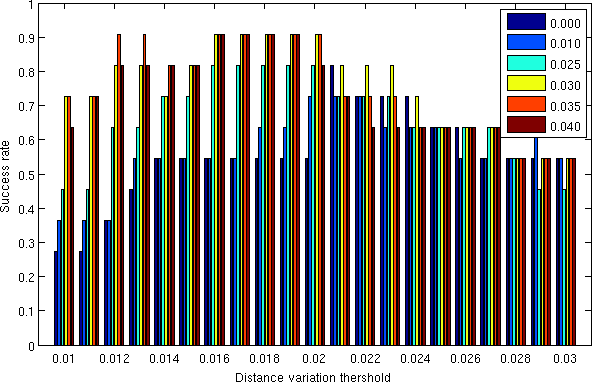
\includegraphics[width=.9\columnwidth]{figures/distribution.png}
		\vspace{-2ex}
   \caption{Clustering success rate on 17 scenes for different values of $p_{threshold}$ (see legend) as a function of $d_{threshold}$ (in meters).}
   \label{fig:clustering}
 \end{center}
 \end{figure}


 

\subsection{Dense Model Reconstruction}
\label{sec:dense_model}

\begin{algorithm}[htb!]\footnotesize
   \tcc{\footnotesize{set of features $F_{clusters}$,
		      distance threshold $d_{roi\_thresh}$,
		      angle threshold $eps_{thresh}$,
		      seed queue $sq$,
		      regions list $R$,
		      current region $R_i$,
		      list of processed points $processed$} }
   \KwIn{$F_{clusters}$, $d_{roi\_thresh}$, $eps_{thresh}$}
   \ForEach {$f_i \in F_{clusters}$}
   {
    $p_{s,i} $:= centroid($f_i$)
    $sq.add(p_{s,i})$
    \tcc{\footnotesize{select a seed point and add it to a queue}}
    $processed(p_{s,i})$ = $true$ \\
    $R_i := \{p_{s,i}\}$
    \tcc{\footnotesize{initialize region}}
    \While {$sq.notempty()$}
    {
      $N := \{q_j \| dist(q_j, R_i[c]) < d_{roi\_thresh}\}$\\
      \tcc{\footnotesize{select neighborhood}}
      \ForEach {$q_j \in N$}
      {
	\If {$processed(q_j)$ = $true$} 
	{
	$continue$
	}
	\If {$boundary(q_j)$ = $true$} 
	{
	$stopgrowing =true$\\
	$R_i \leftarrow R_i \cup \{q_j\}$
	$processed(q_j)$ = $true$ \\
	$break$
	}
		\If { deg ($\vec{p_{s,i}q_j} , norm(q_j)$) $>$ $eps_{thresh}$   }
	{
	 $R_i \leftarrow R_i \cup \{q_j\}$\\
	 $processed(q_j)$ = $true$ \\
	}
	\Else {$break$}
      }
      \If{$stopgrowing = false$ $\&\&$ $\forall q_j \in N\ $boundary($q_j$) = false   }
	{
	$sq \leftarrow N$
	}
    }
    {$R \leftarrow R_i$}
   }
  \ForEach {$R_i, R_j \in R $ }
  {
    \If {$f_i f_j \in $ same object }
	{$R_i \leftarrow R_i \cup \{R_j\}$}
  }
  \KwOut{Dense models $R_{j}$}
  \caption{Region growing with normals \& boundaries.}
  \label{alg:region_growing}
\end{algorithm}

Considering the connected features $F_{clusters}$ as being part of the same object, we reconstruct 
the dense model of the object using region growing in normal space, which also makes use of the 
borders found at depth discontinuities, as shown in %\algref{region_growing}. 
The idea for the region growing 
constraints is based on the segmentation described by Mishra et al.~\cite{asICCV2009}, 
where the authors make use of a predefined fixation point and a border map. Since we already 
know the features that are part of the object, we can easily define a seed point for the
region growing. In order to find the best possible seed point, we separate the connected 
features using euclidean clustering, calculate each of the resulting clusters' centroid, and 
then start growing from these. An important condition of the region growing is the 
assumption that objects are often composed of convex parts~\cite{Pogor}.
Therefore, we make sure that during region growing two points are assigned to the same region $R_{i}$
if the angle $eps_{thresh}$ between the vector connecting them and the points normal is close to obtuse
(considering the sensor noise level\cite{kinect_accuracy}, 89$^\circ$ were used).
Once all region-feature pairs have been identified, we reconstruct the dense model.
Since in the trajectory clustering step we already identified the features that belong to the same object,
having multiple regions for the same object is easily dealt with
by merging those regions for which the corresponding features belong to the same object into dense models $R_{j}$.



\section{Evaluation}
\label{sec:evaluation}
\subsection{Experimental Setup}
The system was evaluated on 17 scenes in different configurations
as illustrated in Fig. \ref{fig:evaluation1}. The   scenes  are   
numbered  1-17 and arranged according to the legend shown in Fig. \ref{fig:table_scenes}.
Though our system can iteratively
cope with multi-object scenes, we performed the evaluation on two-object
scenes with the  finite number  of scene
configurations that  can occur. These configurations  can be split in  three different
ways, namely: i)  size, ii) shape, and iii)  arrangement.  A scene may
consist  of two  objects  of different  sizes  or the  same size.  The
objects may  be either both  flat or round  or a combination  of these
two.  They  may  also  occur  in  different  arrangements;  completely
separated, only  touching, one on  top of the other,  or in solid
contact. Solid  contact refers to  both objects being in  contact with
each  other,  whereby  the  contact  area  is  larger  than  a  single
line (scene   number  4 in Fig. \ref{fig:evaluation1}). Some configurations are
infeasible for our approach.  For example a flat  object and a
round  object cannot  be of the  same  size, or  round object  on top  of
another  round object  cannot be  pushed (one  mug on  top  of another
mug). It is also not possible to  have a round object that is in solid
contact with  another round  object. For this  case we  consider solid
contact as  being two objects touching  with more than  one line, for
example in scene number 17 where also  the handle of the mug  touches the juice box.  

\begin{figure}[ht!]
  \centering 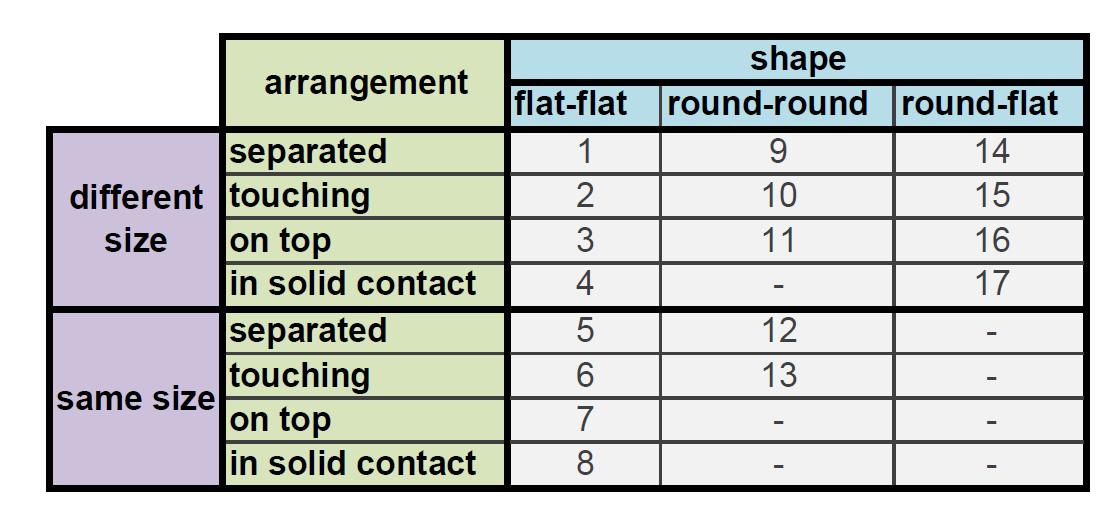
\includegraphics[width=0.8\columnwidth]{figures/table_scenes.png}
  \vspace{-2ex}
  \caption{Legend for the different scene configurations. The scenes are shown in Fig. \ref{fig:evaluation1}.
  }
  \label{fig:table_scenes}
\end{figure}

It is  important to  emphasize that the above  devised conventions 
refer to  the scenes after a  push. The scenes  before interaction were
designed such that it is difficult or impossible to segment
them using static segmentation techniques.
 
Average time to segment one scene from Fig. \ref{fig:evaluation1} amounted to $12.5s$ 
with the pre-segmentation taking $1.5s$, feature extraction $3.5s$, pushing 
$6s$ (tracking runs at $25fps$ for up to 10 features) and dense model reconstruction $1.5s$.
Apart from tracking all modules perform linearly with the
number of  features and objects  respectively and can thus  easily be
used for larger and more complex  scenes. For all the scenes the push
point estimation algorithm was used, the only exception being the 'on
top'  arrangements for which the algorithm does not generalize. 
For this reason and since the scope of the paper is on the priors from
the static segmentation, RGBD features for
textureless objects and the final dense model reconstruction, we performed
the experiments by manually inducing motions into the corners of the scenes.
In  our  future work we  will address  finding a generalized  push point algorithm.
\vspace{-0.5ex}
\subsection{Results}
All  the  experiments were  performed  three  times  for each  of  the
17    scenes.    All    the    results   are    presented    in Tab.
\ref{tab:chart_result} which  shows the segmentation success rate  for every scene. 
The  corresponding figures for this data  can be found in  Fig. \ref{fig:evaluation1}. 
The algorithm was never able to segment the scene number 8 and performed poorly for scenes
6 and 13. In these cases the contact surface of the two objects is large and the objects are of the same size.
Erroneous reconstruction happens due to a lack of a sufficiently good boundary estimation
near the touching surface, and therefore the region growing does not terminate.
This could be alleviated by integrating texture/color-based segmentation methods,
which we plan to investigate in the future.

It  is  important to  note  that  the  overall
segmentation   was    successful   in   more   than    82\%   of   the
experiments.  Tab.\ref{tab:result_percentage}  shows that the more
objects differ  and the less in  contact they are  the more successful
the  segmentation becomes.  Our
algorithm  performs extremely well in the  'on top'  arrangement which  is very
challenging for the static segmentation techniques.

\begin{table}[h!]\scriptsize
\hspace*{-2.5cm} 
\begin{tabular}{|c|c| c| c| c| c| c|c|c|c|c|c|c|c|c|c|c|c|}
\hline    Scene   number    &1   &    2    &   3    &4   &5&6&7&    8&
9&10&11&12&13&14&15&16&17\\ \hline  Success rate[\%] & 100  & 100 &100
&100&100&33,3  & 100  &  0  & 100&  100&  66,7& 100&33,3  &100&100&100
&66,7\\\hline
\end{tabular}
\caption{Segmentation results for  all 17 scenes.  For each scene there  were 3 experiments conducted.}
      \label{tab:chart_result}
\end{table}

\begin{table}[h!]\scriptsize
\hspace*{-4cm} 
\begin{tabular}{|c |c| c| c| c| c| c|c|c|c|}
\hline    &all    results   &    different    size    &   same    size
&flat-flat&round-round&round-flat & apart & in contact (touching or in
solid contact) & on top\\ \hline Success rate[\%] & 82,4 & 93,9 & 61,1
&79,2&80,0&91,7 & 100 & 66,7 & 91,7\\\hline
\end{tabular}
\caption{Segmentation success rates of different scene configurations.
}
\label{tab:result_percentage}
\end{table}

\begin{figure}[h!]  %\renewcommand*{\thesubfigure}{}
  \hspace*{-4.3cm}  
    \begin{tabular}{ccccccccc}
      \hline
      1 & 2 & 3 & 4 & 5 & 6 & 7 & 8 & 9 \\
      \hline
      \hline
    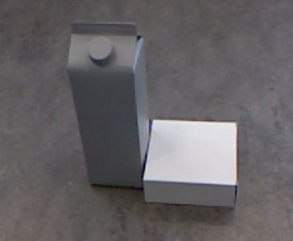
\includegraphics[height=1.5cm]{pictures/11.jpg}&
    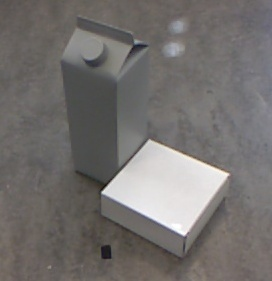
\includegraphics[height=1.5cm]{pictures/21.jpg}&
    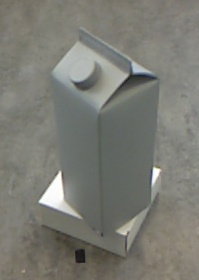
\includegraphics[height=1.5cm]{pictures/31.jpg}&
    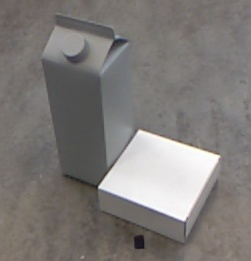
\includegraphics[height=1.5cm]{pictures/41.jpg}&
    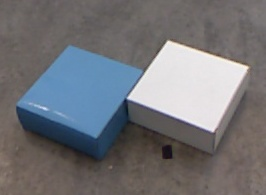
\includegraphics[height=1.5cm]{pictures/51.jpg}&
    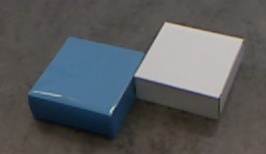
\includegraphics[height=1.5cm]{pictures/61.jpg}&
    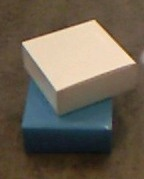
\includegraphics[height=1.5cm]{pictures/71.jpg}&
    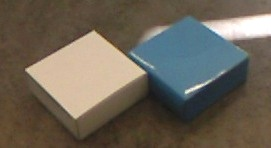
\includegraphics[height=1.5cm]{pictures/81.jpg}&
    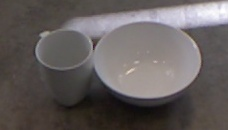
\includegraphics[height=1.5cm]{pictures/91.jpg}\\ 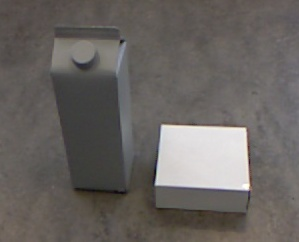
\includegraphics[height=1.5cm]{pictures/12.jpg}&
    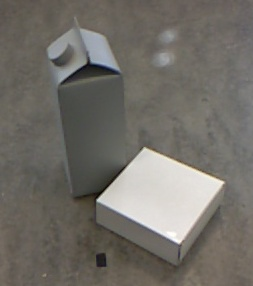
\includegraphics[height=1.5cm]{pictures/22.jpg}&
    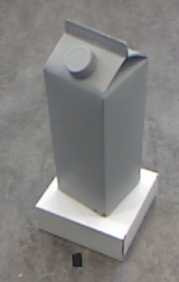
\includegraphics[height=1.5cm]{pictures/32.jpg}&
    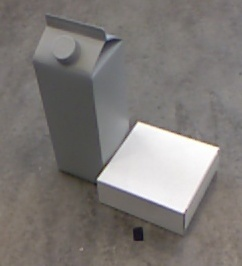
\includegraphics[height=1.5cm]{pictures/42.jpg}&
    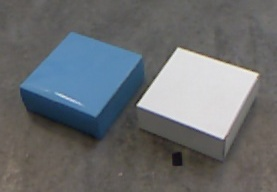
\includegraphics[height=1.5cm]{pictures/52.jpg}&
    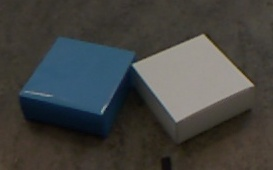
\includegraphics[height=1.5cm]{pictures/62.jpg}&
    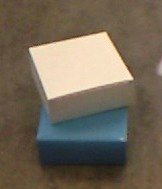
\includegraphics[height=1.5cm]{pictures/72.jpg}&
    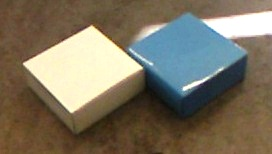
\includegraphics[height=1.5cm]{pictures/82.jpg}&
    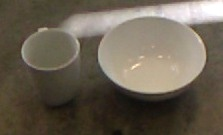
\includegraphics[height=1.5cm]{pictures/92.jpg}\\ 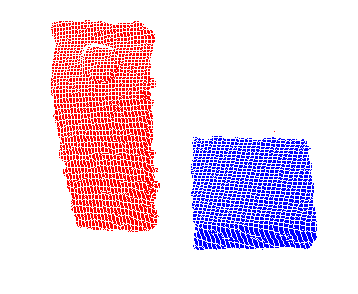
\includegraphics[height=1.5cm]{pictures/13.png}&
    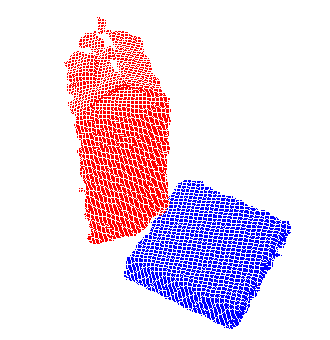
\includegraphics[height=1.5cm]{pictures/23.png}&
    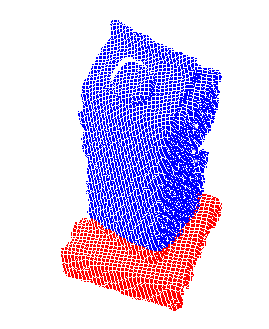
\includegraphics[height=1.5cm]{pictures/33.png}&
    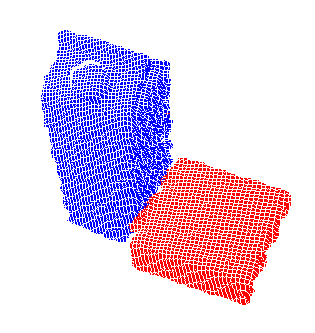
\includegraphics[height=1.5cm]{pictures/43.png}&
    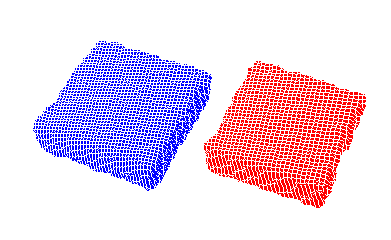
\includegraphics[height=1.5cm]{pictures/53.png}&
    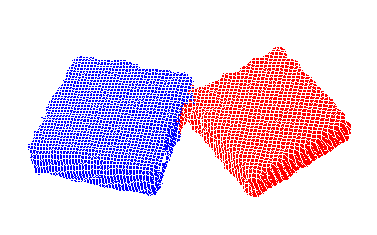
\includegraphics[height=1.5cm]{pictures/63.png}&
    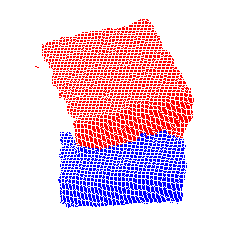
\includegraphics[height=1.5cm]{pictures/73.png}&
    \includegraphics[height=1.5cm]{pictures/83.png}&
    \includegraphics[height=1.5cm]{pictures/93.png}\\
    \end{tabular}
      \hspace*{-3.7cm}  
    \begin{tabular}{cccccccc}
      \hline
      10 & 11 & 12 & 13 & 14 & 15 & 16 & 17\\
      \hline
      \hline
    \includegraphics[height=1.5cm]{pictures/101.jpg}&
    \includegraphics[height=1.5cm]{pictures/111.jpg}&
    \includegraphics[height=1.5cm]{pictures/121.jpg}&
    \includegraphics[height=1.5cm]{pictures/131.jpg}&
    \includegraphics[height=1.5cm]{pictures/141.jpg}&
    \includegraphics[height=1.5cm]{pictures/151.jpg}&
    \includegraphics[height=1.5cm]{pictures/161.jpg}&
    \includegraphics[height=1.5cm]{pictures/171.jpg}\\ \includegraphics[height=1.5cm]{pictures/102.jpg}&
    \includegraphics[height=1.5cm]{pictures/112.jpg}&
    \includegraphics[height=1.5cm]{pictures/122.jpg}&
    \includegraphics[height=1.5cm]{pictures/132.jpg}&
    \includegraphics[height=1.5cm]{pictures/142.jpg}&
    \includegraphics[height=1.5cm]{pictures/152.jpg}&
    \includegraphics[height=1.5cm]{pictures/162.jpg}&
    \includegraphics[height=1.5cm]{pictures/172.jpg}\\ \includegraphics[height=1.5cm]{pictures/103.png}&
    \includegraphics[height=1.5cm]{pictures/113.png}&
    \includegraphics[height=1.5cm]{pictures/123.png}&
    \includegraphics[height=1.5cm]{pictures/133.png}&
    \includegraphics[height=1.5cm]{pictures/143.png}&
    \includegraphics[height=1.5cm]{pictures/153.png}&
    \includegraphics[height=1.5cm]{pictures/163.png}&
    \includegraphics[height=1.5cm]{pictures/173.png}\\
    \end{tabular}
    	\caption{Results  of the  segmentation for  17  scenes.  1st/4th
          image row:  Image before  the push  for scenes.   2nd/5th:
          Image after the push for scenes.  3rd/6th: Point cloud
          after dense model reconstruction for scenes.}
    \label{fig:evaluation1}
\end{figure}

We would  like to draw the  reader's attention to all  the scenes with
the round objects. 
It can be noted that
the Kinect sensor from the used viewpoint (mounted on the head of the human size PR2 robot) always
captures mugs as two spatially non-connected parts.
In order to robustly merge these two parts using segmentation
algorithms operating on point clouds or images of static scenes, 
model-based segmentation algorithms are required. While that constitutes a feasible solution,
the system presented in this
paper can easily deal with such scenes without a model by clustering the two
parts of the mug since they move rigidly with respect to each other.

 For  the scene in  bottom row  of Fig. \ref{fig:scenes}  we can  observe that
 there is only one feature on the left object.  All   the  clustering  algorithms  trying  to
 explicitly cluster  at least one  pair of features with  the constant
 relative  distance over  time would  fail  in this  case.  Using  the
 graph-based clustering method we are able to disconnect the two nodes
 of  the  graph  and infer  that  there  is a single feature-object association.



\section{Conclusion}
\label{sec:conclusion}
We have  presented a novel interactive segmentation  system suitable for
the segmentation of textureless  objects in cluttered tabletop scenes.
Integrated  in the  system are  the static  pre-segmentation  based on
geometrical   categorization,  a  push   point and direction estimation, 
RGBD features  suitable for tracking of
textureless objects,  the graph-based trajectory  clustering algorithm
and the  dense model reconstruction.  A rigorous  evaluation of the
system on a  set of 17 scenes showed successful segmentation in $82\%$ of the cases.  
The results show the applicability of our system
for objects of similar colors,  shapes and sizes on predominantly flat
and  round surfaces.  